\documentclass[final]{beamer}\usepackage[]{graphicx}\usepackage[]{color}
%% maxwidth is the original width if it is less than linewidth
%% otherwise use linewidth (to make sure the graphics do not exceed the margin)
\makeatletter
\def\maxwidth{ %
  \ifdim\Gin@nat@width>\linewidth
    \linewidth
  \else
    \Gin@nat@width
  \fi
}
\makeatother

\definecolor{fgcolor}{rgb}{0.345, 0.345, 0.345}
\newcommand{\hlnum}[1]{\textcolor[rgb]{0.686,0.059,0.569}{#1}}%
\newcommand{\hlstr}[1]{\textcolor[rgb]{0.192,0.494,0.8}{#1}}%
\newcommand{\hlcom}[1]{\textcolor[rgb]{0.678,0.584,0.686}{\textit{#1}}}%
\newcommand{\hlopt}[1]{\textcolor[rgb]{0,0,0}{#1}}%
\newcommand{\hlstd}[1]{\textcolor[rgb]{0.345,0.345,0.345}{#1}}%
\newcommand{\hlkwa}[1]{\textcolor[rgb]{0.161,0.373,0.58}{\textbf{#1}}}%
\newcommand{\hlkwb}[1]{\textcolor[rgb]{0.69,0.353,0.396}{#1}}%
\newcommand{\hlkwc}[1]{\textcolor[rgb]{0.333,0.667,0.333}{#1}}%
\newcommand{\hlkwd}[1]{\textcolor[rgb]{0.737,0.353,0.396}{\textbf{#1}}}%

\usepackage{framed}
\makeatletter
\newenvironment{kframe}{%
 \def\at@end@of@kframe{}%
 \ifinner\ifhmode%
  \def\at@end@of@kframe{\end{minipage}}%
  \begin{minipage}{\columnwidth}%
 \fi\fi%
 \def\FrameCommand##1{\hskip\@totalleftmargin \hskip-\fboxsep
 \colorbox{shadecolor}{##1}\hskip-\fboxsep
     % There is no \\@totalrightmargin, so:
     \hskip-\linewidth \hskip-\@totalleftmargin \hskip\columnwidth}%
 \MakeFramed {\advance\hsize-\width
   \@totalleftmargin\z@ \linewidth\hsize
   \@setminipage}}%
 {\par\unskip\endMakeFramed%
 \at@end@of@kframe}
\makeatother

\definecolor{shadecolor}{rgb}{.97, .97, .97}
\definecolor{messagecolor}{rgb}{0, 0, 0}
\definecolor{warningcolor}{rgb}{1, 0, 1}
\definecolor{errorcolor}{rgb}{1, 0, 0}
\newenvironment{knitrout}{}{} % an empty environment to be redefined in TeX

\usepackage{alltt}
\usepackage{grffile}
\mode<presentation>{\usetheme{CambridgeUSPOL}}

\usepackage[utf8]{inputenc}
\usepackage{amsfonts}
\usepackage{amsmath}
\usepackage{natbib}
\usepackage{graphicx}
\usepackage{array,booktabs,tabularx}
\usepackage{epstopdf}
\usepackage{colortbl, xcolor}
\newcolumntype{Z}{>{\centering\arraybackslash}X}

% rysunki
\usepackage{tikz}
\usepackage{ifthen}
\usepackage{xxcolor}
\usetikzlibrary{arrows}
\usetikzlibrary[topaths]
\usetikzlibrary{decorations.pathreplacing}
%\usepackage{times}\usefonttheme{professionalfonts}  % times is obsolete
\usefonttheme[onlymath]{serif}
\boldmath
\usepackage[orientation=portrait,size=a0,scale=1.4,debug]{beamerposter}                       % e.g. for DIN-A0 poster
%\usepackage[orientation=portrait,size=a1,scale=1.4,grid,debug]{beamerposter}                  % e.g. for DIN-A1 poster, with optional grid and debug output
%\usepackage[size=custom,width=200,height=120,scale=2,debug]{beamerposter}                     % e.g. for custom size poster
%\usepackage[orientation=portrait,size=a0,scale=1.0,printer=rwth-glossy-uv.df]{beamerposter}   % e.g. for DIN-A0 poster with rwth-glossy-uv printer check
% ...
%

\usecolortheme{seagull}
\useinnertheme{rectangles}
\setbeamercolor{item projected}{bg=darkred}
% \setbeamertemplate{enumerate items}[default]
\setbeamertemplate{caption}{\insertcaption} 
\setbeamertemplate{navigation symbols}{}
\setbeamercovered{transparent}
\setbeamercolor{block title}{fg=darkred}
\setbeamercolor{local structure}{fg=darkred}

\setbeamercolor*{enumerate item}{fg=darkred}
\setbeamercolor*{enumerate subitem}{fg=darkred}
\setbeamercolor*{enumerate subsubitem}{fg=darkred}

\setbeamercolor*{itemize item}{fg=darkred}
\setbeamercolor*{itemize subitem}{fg=darkred}
\setbeamercolor*{itemize subsubitem}{fg=darkred}

\newlength{\columnheight}
\setlength{\columnheight}{98.5cm}
\renewcommand{\thetable}{}
\def\andname{,}
\authornote{}

\renewcommand{\APACrefatitle}[2]{}
\renewcommand{\bibliographytypesize}{\footnotesize} 
\renewcommand{\APACrefYearMonthDay}[3]{%
  {\BBOP}{#1}
  {\BBCP}
}
\IfFileExists{upquote.sty}{\usepackage{upquote}}{}
\begin{document}




\date{}
\author{Micha\l{} Burdukiewicz\inst{1}, Piotr Sobczyk\inst{2}, Stefan R\"{o}diger\inst{3}, Pawe\l{} Mackiewicz\inst{1} and Ma\l{}gorzata Kotulska\inst{4}\\
\small{*michalburdukiewicz@gmail.com}}

\institute{\small{\textsuperscript{1}University of Wroc\l{}aw, Department of Genomics, \textsuperscript{2}Wroc\l{}aw University of Science and Technology, Faculty of Pure and Applied Mathematics, \textsuperscript{3}Brandenburg University of Technology Cottbus-Senftenberg, Institute of Biotechnology, \textsuperscript{4}Wroc\l{}aw University of Science and Technology, Department of Biomedical Engineering}
}
}
\title{\huge AmyloGram:a novel predictor of amyloidogenicity}

\begin{frame}
\begin{columns}
\begin{column}{.50\textwidth}
\begin{beamercolorbox}[center,wd=\textwidth]{postercolumn}
\begin{minipage}[T]{.95\textwidth}
\parbox[t][\columnheight]{\textwidth}
{
\begin{block}{Introduction}

Amyloids are proteins associated with the number of clinical disorders (e.g., Alzheimer's, Creutzfeldt-Jakob's and Huntington's diseases). Despite their diversity, all amyloid proteins can undergo aggregation initiated by 6- to \mbox{15-residue} segments called hot spots. To find the patterns defining the hot-spots, we trained multiple predictors of amyloidogenicity based on random forests using short subsequences (n-grams) extracted from amyloidogenic and non-amyloidogenic peptides collected in the AmyLoad database. 

\bigskip

The best-performing predictor, AmyloGram, was compared to state-of-art predictors of amyloids using the independent benchmark dataset. 

    \end{block}

\begin{block}{Training of AmyloGram}
\begin{figure} 
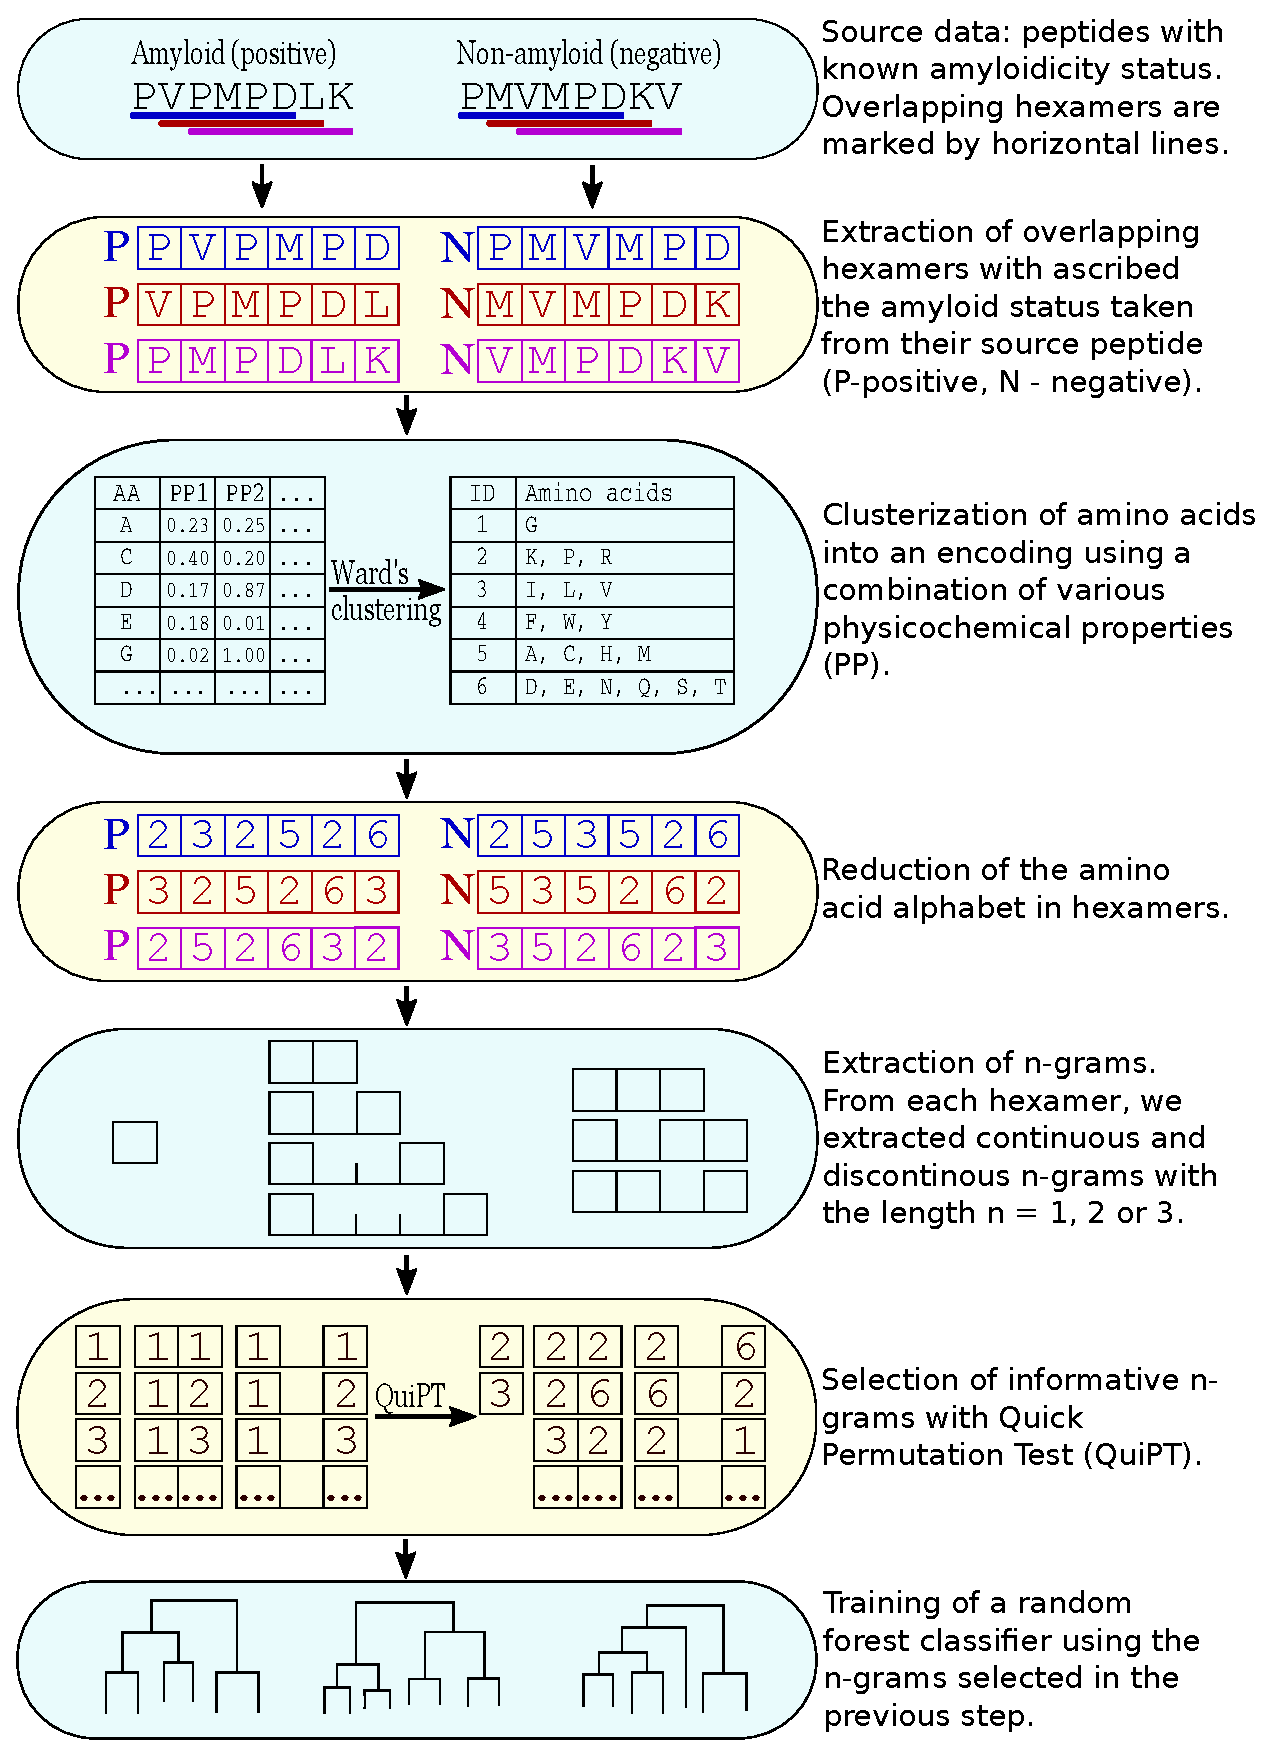
\includegraphics[width=0.85\columnwidth]{static_figure/ngram_scheme_poster.eps}
\end{figure}

    \end{block}


\begin{block}{Reduced amino acid alphabet}

The amyloidogenicity of a given peptide may not depend on the exact sequence of 
amino acids but on its more general properties. We 
handpicked 17 measures from AAIndex database 
describing features important in the amyloidogenicity, such as: size of 
residues, hydrophobicity, solvent surface area, frequency in $\beta$-sheets and 
contactivity. Based on that we created 524,284 amino acid reduced alphabets with different level of 
amino acid alphabet reduction from three to six amino acid groups.

    \end{block}

\begin{block}{Results of cross-validation}

Distribution of mean AUC values of classifiers with various reduced alphabets 
for every possible combination of training and testing data set including 
different lengths of sequences. 

\begin{knitrout}
\definecolor{shadecolor}{rgb}{0.969, 0.969, 0.969}\color{fgcolor}

{\centering 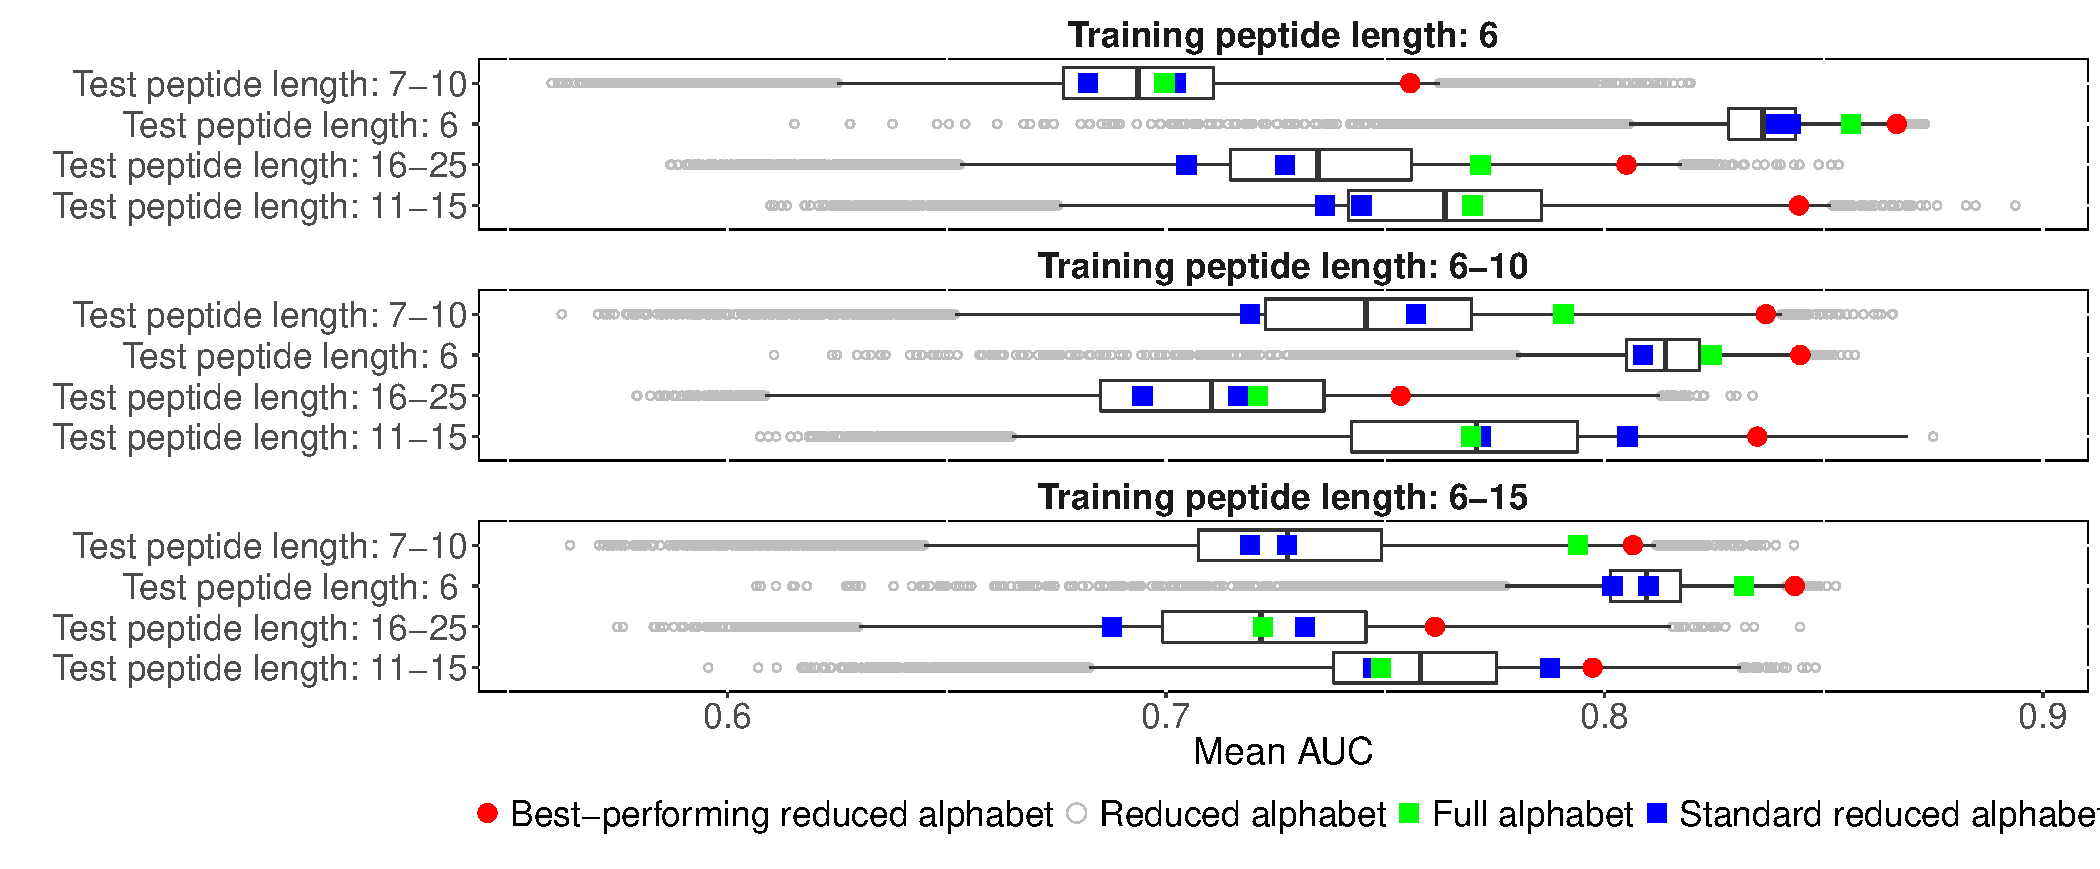
\includegraphics[width=\maxwidth]{figure/unnamed-chunk-1-1} 

}



\end{knitrout}

\tiny
The left and right hinges of boxes correspond to 
the 0.25 and 0.75 quartiles. The bar inside the box represents the median. The 
gray circles correspond to the reduced alphabets with the AUC outside the 0.95 
confidence interval.

\end{block}
\vfill




}
\end{minipage}
\end{beamercolorbox}
\end{column}


%new column ------------------------------------------------------    

\begin{column}{.51\textwidth}
\begin{beamercolorbox}[center,wd=\textwidth]{postercolumn}
\begin{minipage}[T]{.95\textwidth}  
\parbox[t][\columnheight]{\textwidth}
{


\begin{block}{Similarity index}
\begin{knitrout}
\definecolor{shadecolor}{rgb}{0.969, 0.969, 0.969}\color{fgcolor}

{\centering 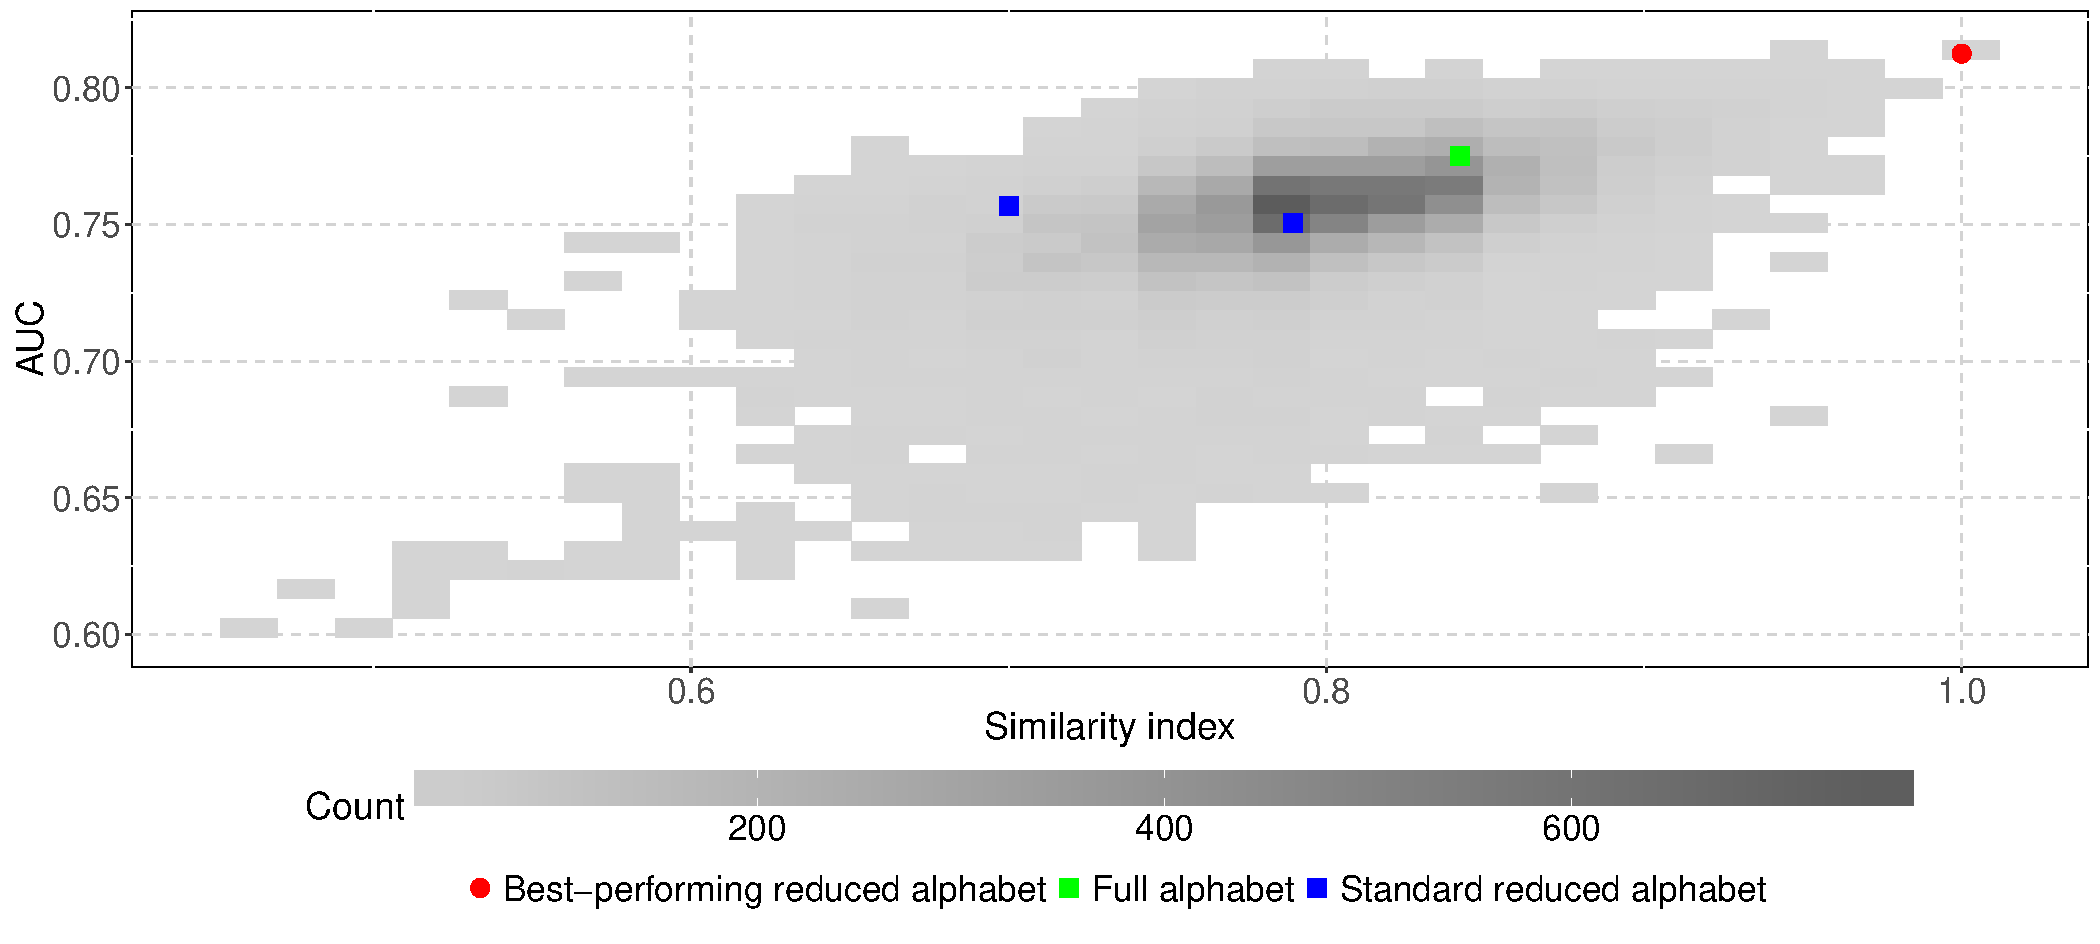
\includegraphics[width=\maxwidth]{figure/unnamed-chunk-2-1} 

}



\end{knitrout}
Similarity index~\citep{stephenson_unearthing_2013} measures the similarity between two reduced alphabets (1 - identical, 0, totally dissimilar). The similarity of a reduced alphabet to the best-performing alphabet is significantly correlated to the AUC of a classifier that employs it. Such relationship indicates that the best-performing reduced alphabet was not found by chance, but represents properties required for the proper prediction of amyloids. 

\end{block}
\vfill




\begin{block}{Informative n-grams}
\begin{knitrout}
\definecolor{shadecolor}{rgb}{0.969, 0.969, 0.969}\color{fgcolor}

{\centering 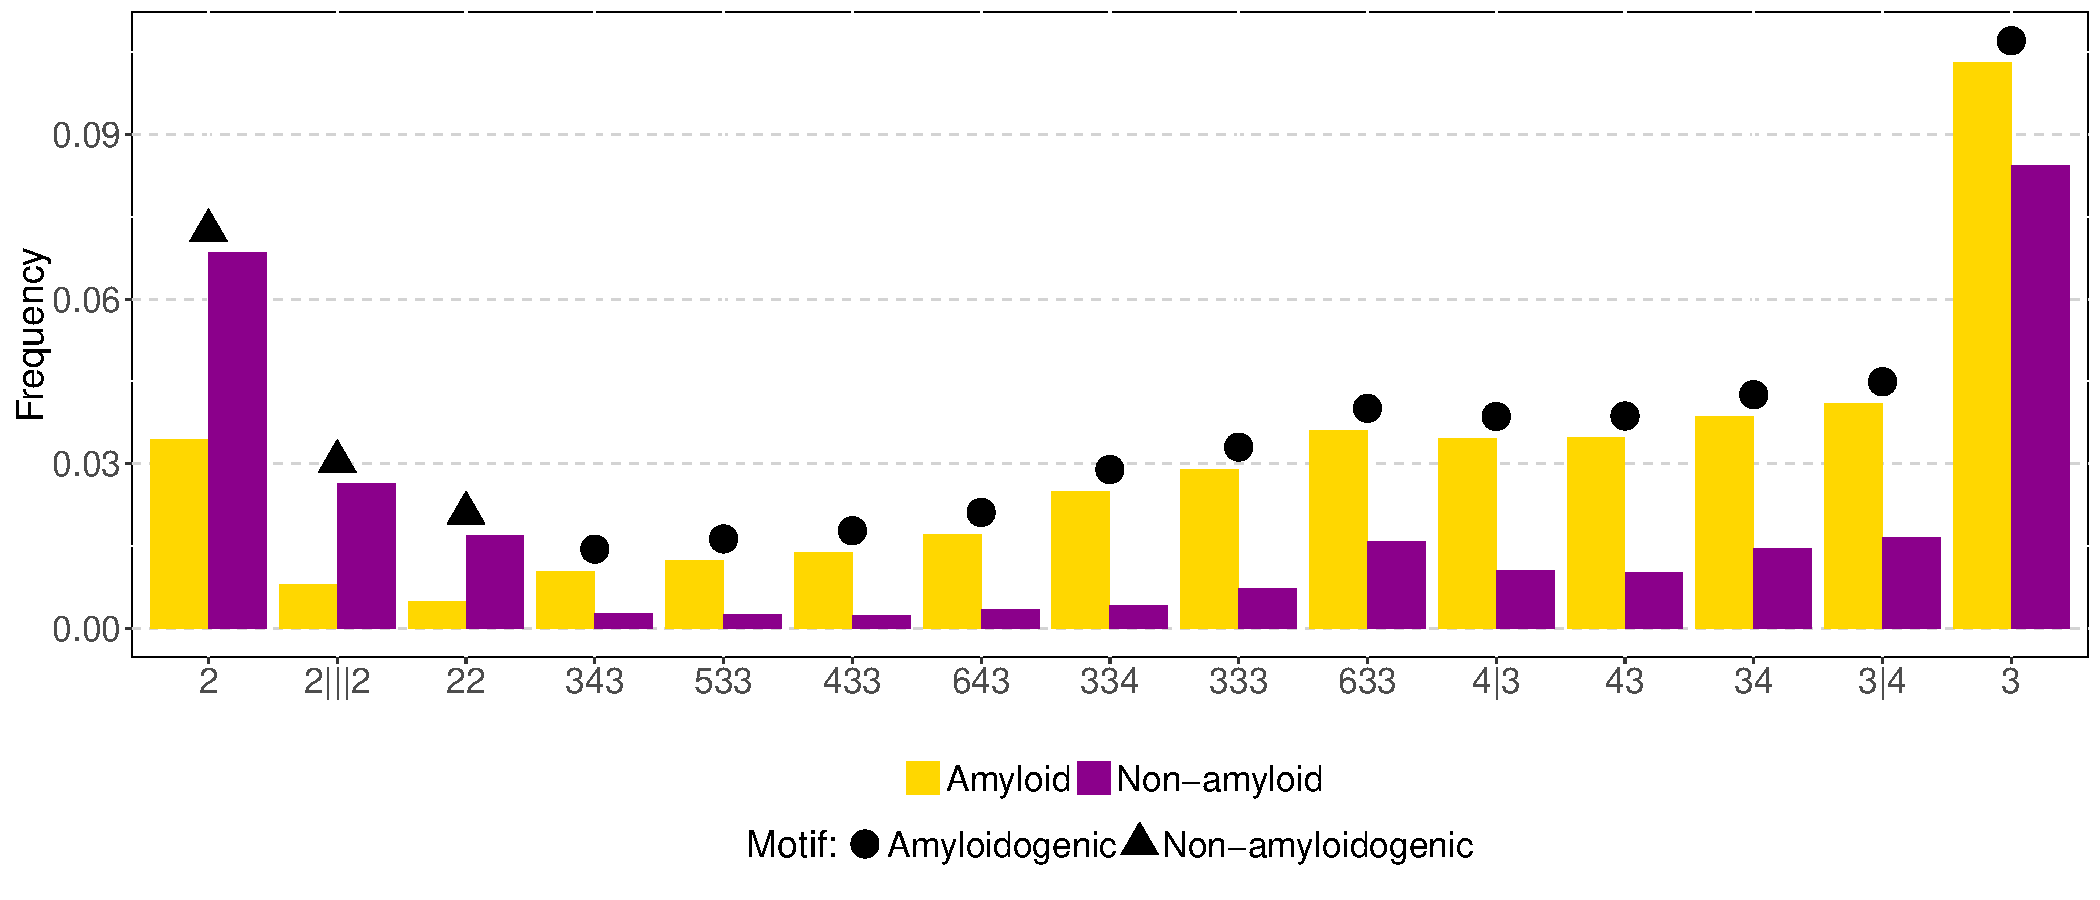
\includegraphics[width=\maxwidth]{figure/unnamed-chunk-3-1} 

}



\end{knitrout}

The frequency of important n-grams used by the best-performing 
classifier in amyloid and non-amyloid sequences. The elements of n-grams are 
amino acids encoded using the best-performing reduced amino acid alphabet. 
A vertical bar represents a gap in a n-gram between 
its elements. Dots and triangles 
denote n-grams occurring in motifs found in respectively amyloidogenic and 
non-amyloidogenic sequences~\citep{paz_sequence_2004}.

\end{block}
\vfill



\begin{block}{Benchmark results}

\begin{table}[ht]
\centering

\begin{tabular}{ccccc}
  \toprule
Classifier & AUC & MCC & Sensitivity & Specificity \\ 
  \midrule
AmyloGram & \textbf{0.8972} & \textbf{0.6307} & 0.8658 & 0.7889 \\ 
  \rowcolor{white}PASTA 2.0\citep{walsh_pasta_2014} & 0.8550 & 0.4291 & 0.3826 & 0.9519 \\ 
   FoldAmyloid \citep{garbuzynskiy_foldamyloid:_2010} & 0.7351 & 0.4526 & 0.7517 & 0.7185 \\ 
  \rowcolor{white}APPNN \citep{familia_prediction_2015} & 0.8343 & 0.5823 & \textbf{0.8859} & 0.7222 \\ 
   \bottomrule
\end{tabular}
\end{table}

The predictor based on the best-performing alphabet, called AmyloGram, was benchmarked against the most popular tools for the detection of amyloid peptides using an external data set \textit{pep424}.

\end{block}
\vfill



\begin{block}{Summary}

We identified a group of reduced amino acid alphabets which capture properties of amyloids. 

\bigskip

Classifiers based on the full (i.e., unreduced) amino acid alphabet never predicted 
amyloidogenicity better than the best classifier based on the reduced alphabet.

\bigskip

Our algorithm was also capable of extracting n-gram associated with amyloidogenicity, partially confirming experimental results.


\end{block}
\vfill


\begin{block}{Availability and funding}

Our software is available as a web-server: \url{smorfland.uni.wroc.pl/amylogram}.

\bigskip

\small{This research was partially funded by the KNOW Consortium and National Science Center (2015/17/N/NZ2/01845).}

\end{block}
\vfill

 \begin{block}{Bibliography}
  \tiny{
  \bibliographystyle{apalike}
  \bibliography{references}
  }
  \end{block}
  \vfill  


}
\end{minipage}
\end{beamercolorbox}
\end{column}
\end{columns}  
\end{frame}
\end{document}
